\documentclass{beamer}
 
\usepackage[utf8]{inputenc}
\usepackage{amsmath}
\usepackage{amssymb}
 
 
%Information to be included in the title page:
\title{Combinatorics: Introduction}
\author{Ben Kettle}
\date{10 Jan 2020}
 
\begin{document}
 
\frame{\titlepage}
 
\begin{frame}
\frametitle{What is combinatorics?}
Combinatorics is an area of math that focuses on methods of counting. It allows us to handle problems that are not immediately solvable by breaking them into parts that we can understand.
\end{frame}

\begin{frame}{Size of a Set}
In combinatorics, we'll be dealing with \alert{sets} a whole lot, especially with the \alert{size} of those sets. \newline
 
\textbf{Definition:} Set \newline
A set is simply a collection of distinct elements. For example, the set of primary colors: $C = \{"red", "green", "blue", "yellow"\}$. \newline

We signify the size of a set with vertical bars, like absolute value. $|C| = |\{"red", "green", "blue", "yellow"\}| = 4$
    
\end{frame}

\begin{frame}{Notation \& Sum Rule}
\only<1-2>{Let’s say we want to find a snack. There are 5 snacks in the fridge and 4 snacks on the counter. How many total snack options do we have, if we assume that any one snack is not both in the fridge and on the counter?}
\newline\newline

\only<2>{9. Here, we essentially want to find the set of ALL snacks, whether on the counter or in the fridge. Because no one item is in both places, we can simply add the two original sizes to find the size of the larger set.}

\only<3-4>{
    In mathematical terms, the \textbf{union} of any number of sets $A, B, C\ldots$ is the set $S$ of all the elements that are in any of those sets.
    We write this mathematically as $A \cup B \cup C \cup \ldots$
    \newline
    For example, given:
    \[ C = \{ "red", "green", "blue", "yellow"\},\ D = \{ "orange", "purple"\} \]
} 
\only<3>{
    \[C \cup D = \ ?\] 
    \[|C \cup D| = \ ?\]
}
\only<4>{
    \[C \cup D = \{ "red", "green", "blue", "yellow", "orange", "purple"\}  \] 
    \[|C \cup D| = 6\]
    
    Be careful! If $E=\{"yellow", "pink"\}$, then $C\cup E = \{ "red", "green", "blue", "yellow", "pink"\}$ and $|C\cup E| = 5.$
}

\only<5>{
    \textbf{Def:} Disjoint Sets \newline
    For sets to be disjoint, they must have no elements in common. $\{1,2\}$ and $\{3,4\}$ are disjoint, but $\{1,2\}$ and $\{1,3\}$ are not.
    \newline\newline
    \textbf{Rule of Sum:} If $A_1, A_2, \ldots, A_n$ are disjoint, then $|A_1 \cup A_2 \cup \cdots \cup A_n = |A_1| + |A_2| + \cdots + |A_n|$
}
\end{frame}

\begin{frame}{Rule of Sum: Exercises}
\begin{enumerate}
    \item Define $A = {1,2,3,4}$ and $B = {2,4,6,8}$. What is $A\cup B$? $|A \cup B|$?
    \item Set $S_1$ has 100 elements, and set $S_2$ has 65 elements. 8 elements are in both $S_1$ and $S_2$. What is $|S_1 \cup S_2|$?
\end{enumerate}
\end{frame}

\begin{frame}{Product Rule}
    \only<1>{
    Suppose instead of a snack, we now want to pick a lunch consisting of a food item and a drink. In our kitchen, we have:
    \begin{center}
        \begin{tabular}{cc}
        \textbf{food} & \textbf{drinks} \\
        sandwich & apple juice \\
        salad & water \\
        pizza & milk \\
        cheetos & \\
        \end{tabular}
    \end{center}
    
    How many different lunch options do we have?
    }
    
    \only<2>{
    To make sense of this intuitively, it's good to make a tree. Our sandwich must include a food item, so let's start with that. How many food options did we have?
    }
    \includegraphics<3>[scale=.3]{lunchtree1.png}
    \includegraphics<4>[scale=.3]{lunchtree2.png}
    \includegraphics<5>[scale=.3]{lunchtree3.png}
    
    \only<6-7>{We can see that there are 12 total lunch options. But that was a lot of work. What might be an easier way than making a tree?}\newline
    
    \only<7>{As you might've guessed from the title of these slides, we can just multiply. We were given 4 food options and 3 drink options, and indeed, $4\cdot 3 = 12$ total lunch options.}
    
    \only<8-10>{Now let's think about this in terms of sets. What is the set that we're counting here?
    \visible<9-10>{\newline\newline We want the size of the set of all lunches---pairs of a food item and a drink item. If we define $L$ as the set of lunches:
    
    \[L = \left\{\begin{array}{c}
        (sandwich, apple\ juice), \\
        (sandwich, water), \\
        \vdots \\
        (cheetos, milk)
    \end{array} \right\} \]
    
    What is $|L|$ in terms of the set of food items $F$ and the set of drinks $D$?
    }
    \visible<10>{\[ |L| = |F|\cdot|D|\]}
    }
    
\end{frame}

\begin{frame}{Product Rule: Formal Definition}

Let's formalize this, and put it into math terms.\newline\newline
\visible<1->{\textbf{Definition:} Cartesian Product
    
    If $S_1, S_2, \ldots, S_n$ are sets, then $S_1 \times S_2 \times \cdots \times S_n$ is the set of all sequences with the first element drawn from $S_1$, the second element from $S_2$, and so on. For example, $L = F \times D$ on the last slide.}
\newline\newline
\visible<2->{\textbf{Definition:} Product Rule

    If $P_1, P_2, \ldots, P_n$ are \alert{sets}, then $|P_1 \times P_2 \times \cdots \times P_n| = |P_1| \cdot |P_2| \cdots |P_n|$.
    }
\end{frame}

\begin{frame}{Product Rule: Exercises}
    \begin{enumerate}
        \item You have been wanting pets for a long time, and finally decide to get a dog, a cat, and a fish. At the pet store, they have 7 dogs, 3 cats, and 3 fish. How many different sets of pets can you bring home? \visible<2>{\alert{$7\cdot 3 \cdot 3 = 63$ options}}
        
        \item For dinner, you can have either a full meal or McDonalds. For the meal, you have 3 salad options and 8 main dish options. At McDonalds, there 10 sandwich options, and 3 sizes of fries. How many total dinner options do you have?
        \visible<2>{\alert{$3\cdot 8 + 10 \cdot 3 = 54$}}
    \end{enumerate}
\end{frame}

\begin{frame}{Product Rule: More Exercises}
    \begin{enumerate}
    \setcounter{enumi}{2}
    \item Getting dressed in the morning, you need shoes, pants, a shirt, and a jacket. Your closet has 4 shoes, 5 pants, 8 shirts, and 3 jackets. However, you have one pair of black shoes and one pair of dark blue pants that you can't wear together. How many outfits can you wear?\newline
    
    \visible<2>{\alert{$4\cdot 5 \cdot 8 \cdot 3 = 480$ total, but we must exclude the outfits with black shoes and black pants. With black shoes and black pants, there are $1$ black pants $\cdot 1$ black shoes $\cdot$ $8$ shirts $\cdot$ $3$ jackets = $24$ outfits.\newline
    
    480 total - 24 unwearable = 456 possible outfits}}
    \end{enumerate}
\end{frame}

\begin{frame}{Counting Subsets}
    \textbf{Definition:} Subset
    
    A subset is a set who's elements are completely contained within another set. We signify this with the $\subseteq$ sign. For example, $\{1,2,3\}$ is a subset of $\{1,2,3,4\}$, so we can say $\{1,2,3\} \subseteq \{1,2,3,4\}$. Similarly, $\{1,2,3\} \subseteq \mathbb{N}$ and $\{3.14, \tfrac{22}{7}, \pi\} \subseteq \mathbb{R}$.\newline
    
    How many subsets of the set $\{a,b,c\}$ are there? What are they?
    
    \visible<2>{\alert{
        The subsets of $\{a,b,c\}$ are:
        \[
        \begin{array}{cccc}
        \varnothing \text{ (empty set)} & \{a\} & \{b\} & \{a,b\} \\
        \{c\} & \{a,c\} & \{b,c\} & \{a,b,c\}
        \end{array}
        \] For a total of 8 subsets.
    }}
\end{frame}

\begin{frame}{Counting Subsets: Bijections}
    There must be an easier way to count these, right? Now, we get to one of the core principles of combinatorics: counting one set by counting another set of the same size. To do this, we must understand what \alert{bijections} are.\newline
    
    \visible<2->{
    \textbf{Definition:} Bijection\newline
    There exists a bijection between two sets if there is a one-to-one mapping from each element in the first set to a unique element in the second set. As a result, if there is a bijection from $A$ to $B$, then $|A| = |B|$. This is very useful! \newline}
    
    \visible<3->{
    Can anyone think of a bijection we might use to count the number of subsets of a set $S$? \visible<4>{\textit{Hint: each element in $S$ must either be included in the subset or not included in the subset}}
    }
\end{frame}

\begin{frame}{Counting Subsets: Bijections}
    We're looking for a way to map each subset of a set $S$ to an element of some other set. \visible<2->{Because each element in $S$ must either be in the subset or out of the subset, we can assign each element in $S$ a 1 (in the subset) or a 0 (out of the subset). Thus, for an $n$-element set $S$, an $n$-bit \alert{binary sequence}, or sequence of 1s and 0s, corresponds to a single subset of $S$.\newline}
    
    \visible<3->{For example, for the set $S=\{x_1, x_2, \ldots, \x_10\}$, the subset $\{x_2, x_3, x_5, x_7, x_10\}$ maps to the sequence 0110101001.
    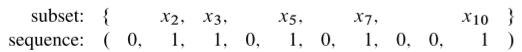
\includegraphics[scale=.9]{binseqmap.png}\newline}
    
    \visible<4->{Try it: for the same set $S$, which subset maps to the sequence 0101000101?   \visible<5->{\alert{$\{x_2,x_4,x_8,x_{10}\}$}}}
\end{frame}

\begin{frame}{Counting Subsets: Bijections - Example}

We determined earlier that there exist 8 subsets of a 3-element set. Let's write out the mapping for those subsets:

\begin{center}
    \begin{tabular}{cc}
        \textbf{sequence} & \textbf{subset} \\
        000 & \visible<2>{\varnothing} \\
        001 & \visible<2>{\{x_1\}} \\
        010 & \visible<2>{\{x_2\}} \\
        011 & \visible<2>{\{x_2,x_3\}} \\
        100 & \visible<2>{\{x_1\}} \\
        101 & \visible<2>{\{x_1,x_3\}} \\
        110 & \visible<2>{\{x_1,x_2\}} \\
        111 & \visible<2>{\{x_1,x_2,x_3\}}
    \end{tabular}
\end{center}
We can see clearly that each sequence maps to one and only one subset here.
\end{frame}

\begin{frame}{Counting Subsets: Bijections}

If every $n$-bit binary sequence corresponds to a single subset, what can we say about the number of subsets of an $n$-element set? \textit{hint: how many n-bit sequences exist?}\newline

\visible<2->{We can use the product rule to find this. To find every possible $n$-bit binary sequence, we want to select one item each from $n$ sets of $\{0,1\}$. In other words, the first position can be either 0 or 1, the second position can be either 0 or 1, etc. Thus, there are $2^n$ $n$-bit binary sequences. Because there is a bijection from these sequences to subsets, this means that there are also $2^n$ subsets of an $n$-element set.}\newline

\visible<3>{If $S$ is a set containing $n$ elements, there are $2^n$ possible subsets of $S$.}
    
\end{frame}

\begin{frame}{Exercises}
\begin{enumerate}
    \item If a certain website requires passwords of two letters, followed by 8 digits. For example, AB12345678 would be a valid password. How many possible passwords exist?
    
    \item If we have the same password requirements, but no repetition is allowed, how many password options are there? 
    
\end{enumerate}
\end{frame}
 
\end{document}